\title{Моделирование структуры абрикосовских вихрей в сверхпроводниках 
    типа 1,5}
\author{Голубев А.В.}
\institute{ВолгГТУ}
\date{}

\begin{frame}
    \titlepage
\end{frame}

\begin{frame}
    \frametitle{Цель}
    \begin{itemize}
        \item исследование появления сверхпроводимости типа 1,5;
        \item исследования случая многополосной сверхпроводимости;
        \item теоретический анализ модели;
        \item моделирование структуры абрикосовских вихрей;
    \end{itemize}
\end{frame}

\begin{frame}
    \frametitle{Актуальность работы}
    \begin{itemize}
        \item широкие возможностями применения сверхпроводников в 
            современной микроэлектронике;
        \item перспективность в исследовании смешанного состояния;
        \item малая изученность физики данного процесса;
        \item высокотемпературные сверхпроводники;
    \end{itemize}
\end{frame}

\begin{frame}
    \frametitle{Фазовая диаграмма}
    \begin{figure}[h]
        \center
        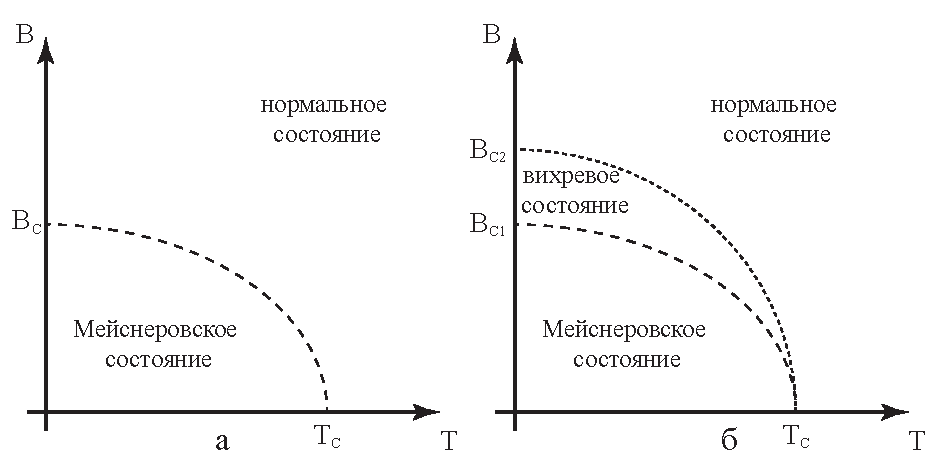
\includegraphics[width=0.7\linewidth]{img_01}
        \caption{Фазовая диаграмма состояния сверхпроводников 1-го (а) и 
            2-го (б) рода}
    \end{figure}
\end{frame}

\begin{frame}
    \frametitle{Фазовая диаграмма магнитных фаз}
    \begin{figure}[h]
        \center
        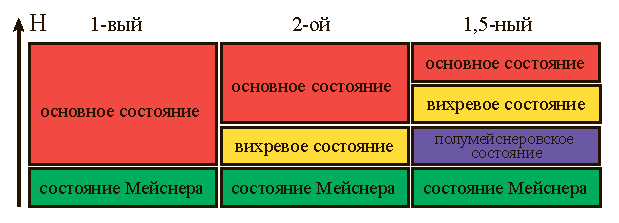
\includegraphics[width=0.7\linewidth]{1-01}
        \caption{Сравнение фазовых диаграмм магнитных фаз чистых 
            сверхпроводников первого, второго и полуторного рода при нулевой 
            температуре.}
    \end{figure}
\end{frame}

\begin{frame}
    \frametitle{Двухкомпонентная модель Гинзбурга-Ландау}
    \begin{gather}
        F = \frac{1}{2}(D\psi_1)(D\psi_1)^* + 
            \frac{1}{2}(D\psi_2)(D\psi_2)^* -
            \nu Re\left( (D\psi_1)(D\psi_2)^* \right) + \nonumber \\ +
            \frac{1}{2}\left(\nabla\times\vec{A}\right)^2 + F_p
    \end{gather}
    Здесь \( D = \nabla + ie\vec{A} \) и \( \psi_a = |\psi_a|e^{i\theta_a} \), 
    \( a = 1,2 \).
\end{frame}

\begin{frame}
    \frametitle{Моделирование структуры вихрей}
\end{frame}

\begin{frame}
    \frametitle{Результаты}
    \begin{figure}[h]
        \begin{minipage}[h]{0.49\linewidth}
            \center{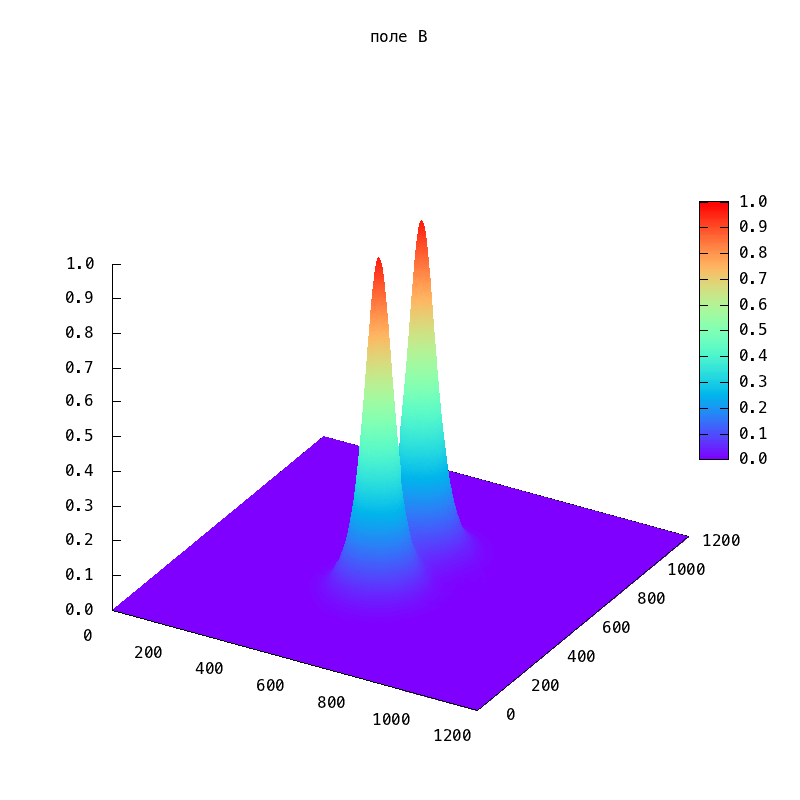
\includegraphics[width=0.7\linewidth]{3d_B}}
        \end{minipage}
        \hfill
        \begin{minipage}[h]{0.49\linewidth}
            \center{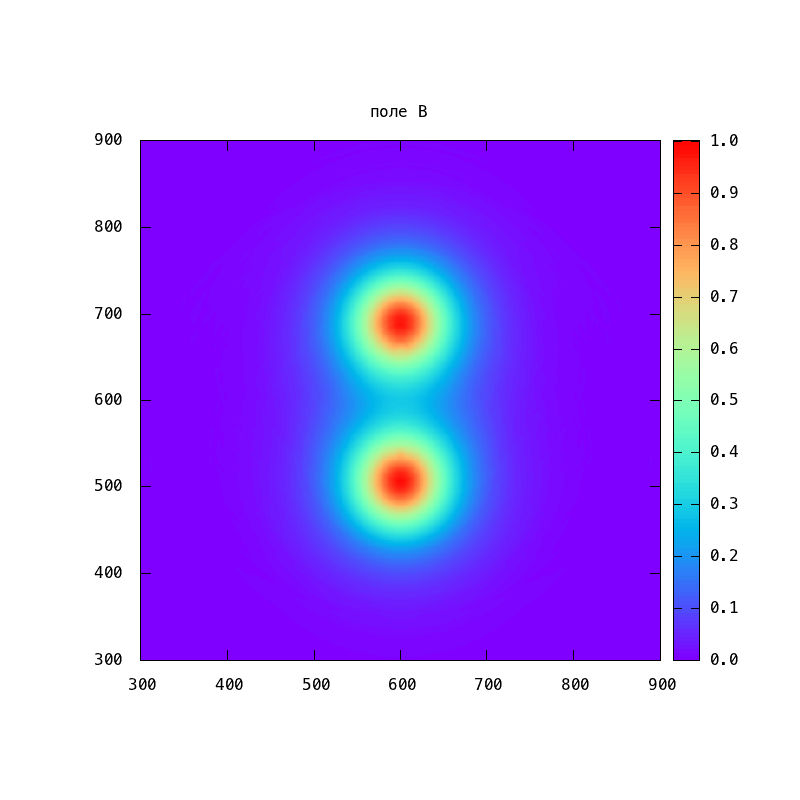
\includegraphics[width=0.7\linewidth]{map_B}}
        \end{minipage}
        % \caption{Распределение магнитного поля в сверхпроводнике}
    \end{figure}
\end{frame}

\begin{frame}
    \frametitle{Результаты}
    \begin{figure}[h]
        \begin{minipage}[h]{0.49\linewidth}
            \center{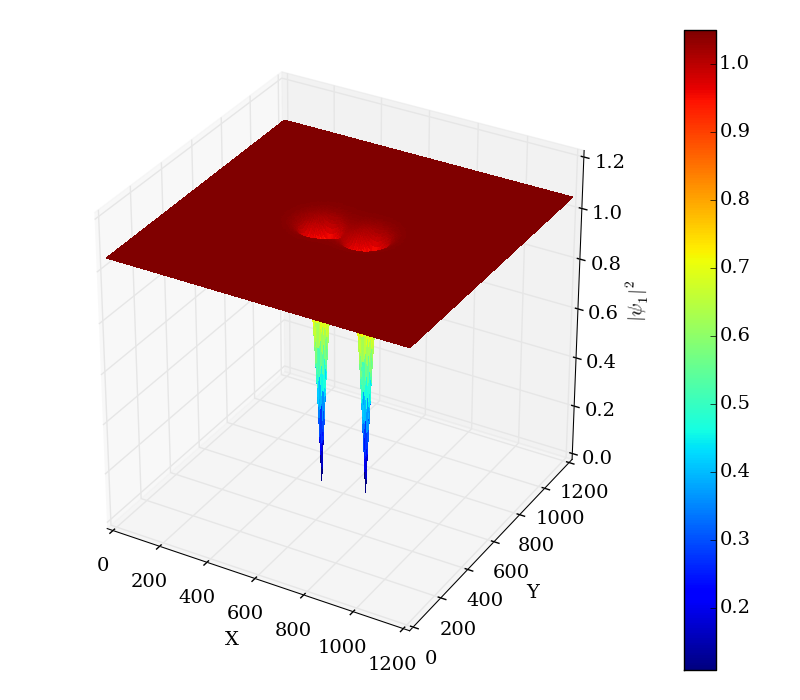
\includegraphics[width=0.7\linewidth]{3d_F1}}
        \end{minipage}
        \hfill
        \begin{minipage}[h]{0.49\linewidth}
            \center{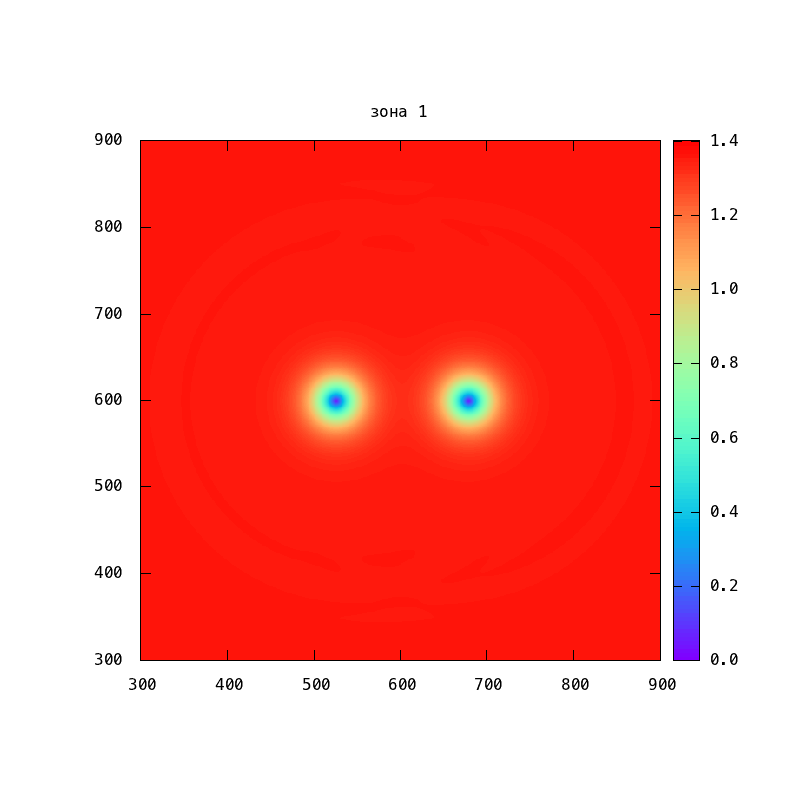
\includegraphics[width=0.7\linewidth]{map_F1}}
        \end{minipage}
        % \caption{}
    \end{figure}
\end{frame}

\begin{frame}
    \frametitle{Результаты}
    \begin{figure}[h]
        \begin{minipage}[h]{0.49\linewidth}
            \center{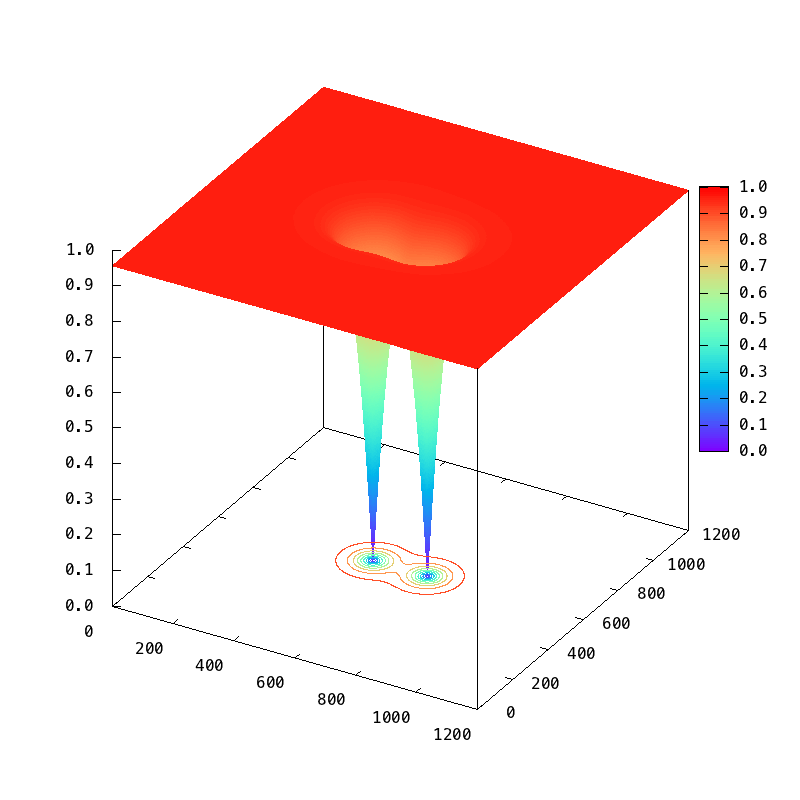
\includegraphics[width=0.7\linewidth]{3d_F2}}
        \end{minipage}
        \hfill
        \begin{minipage}[h]{0.49\linewidth}
            \center{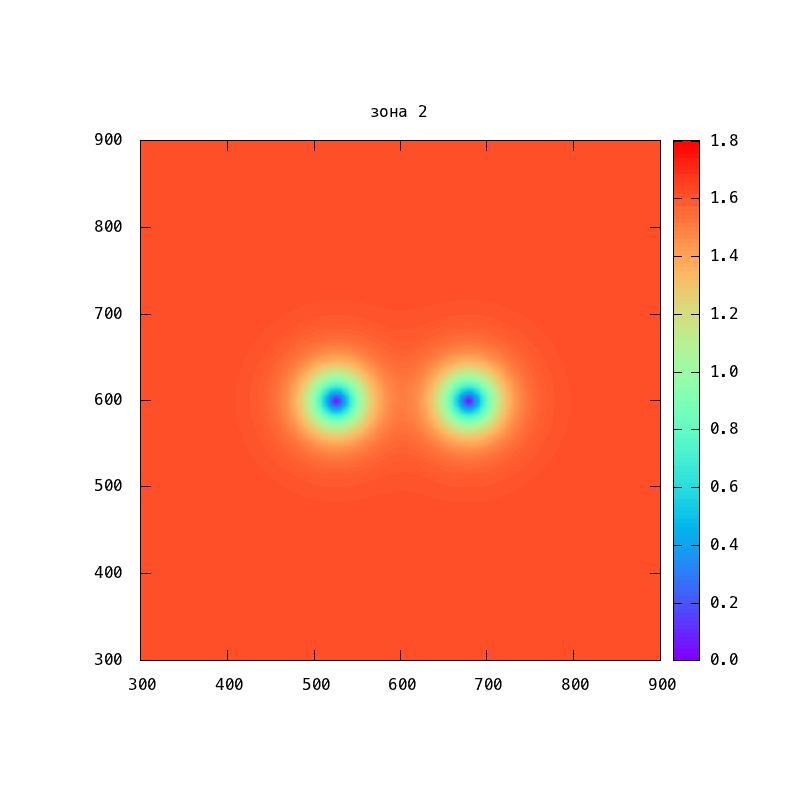
\includegraphics[width=0.7\linewidth]{map_F2}}
        \end{minipage}
        % \caption{}
    \end{figure}
\end{frame}

\begin{frame}
    \frametitle{Результаты}
    \begin{figure}[h]
        \center
        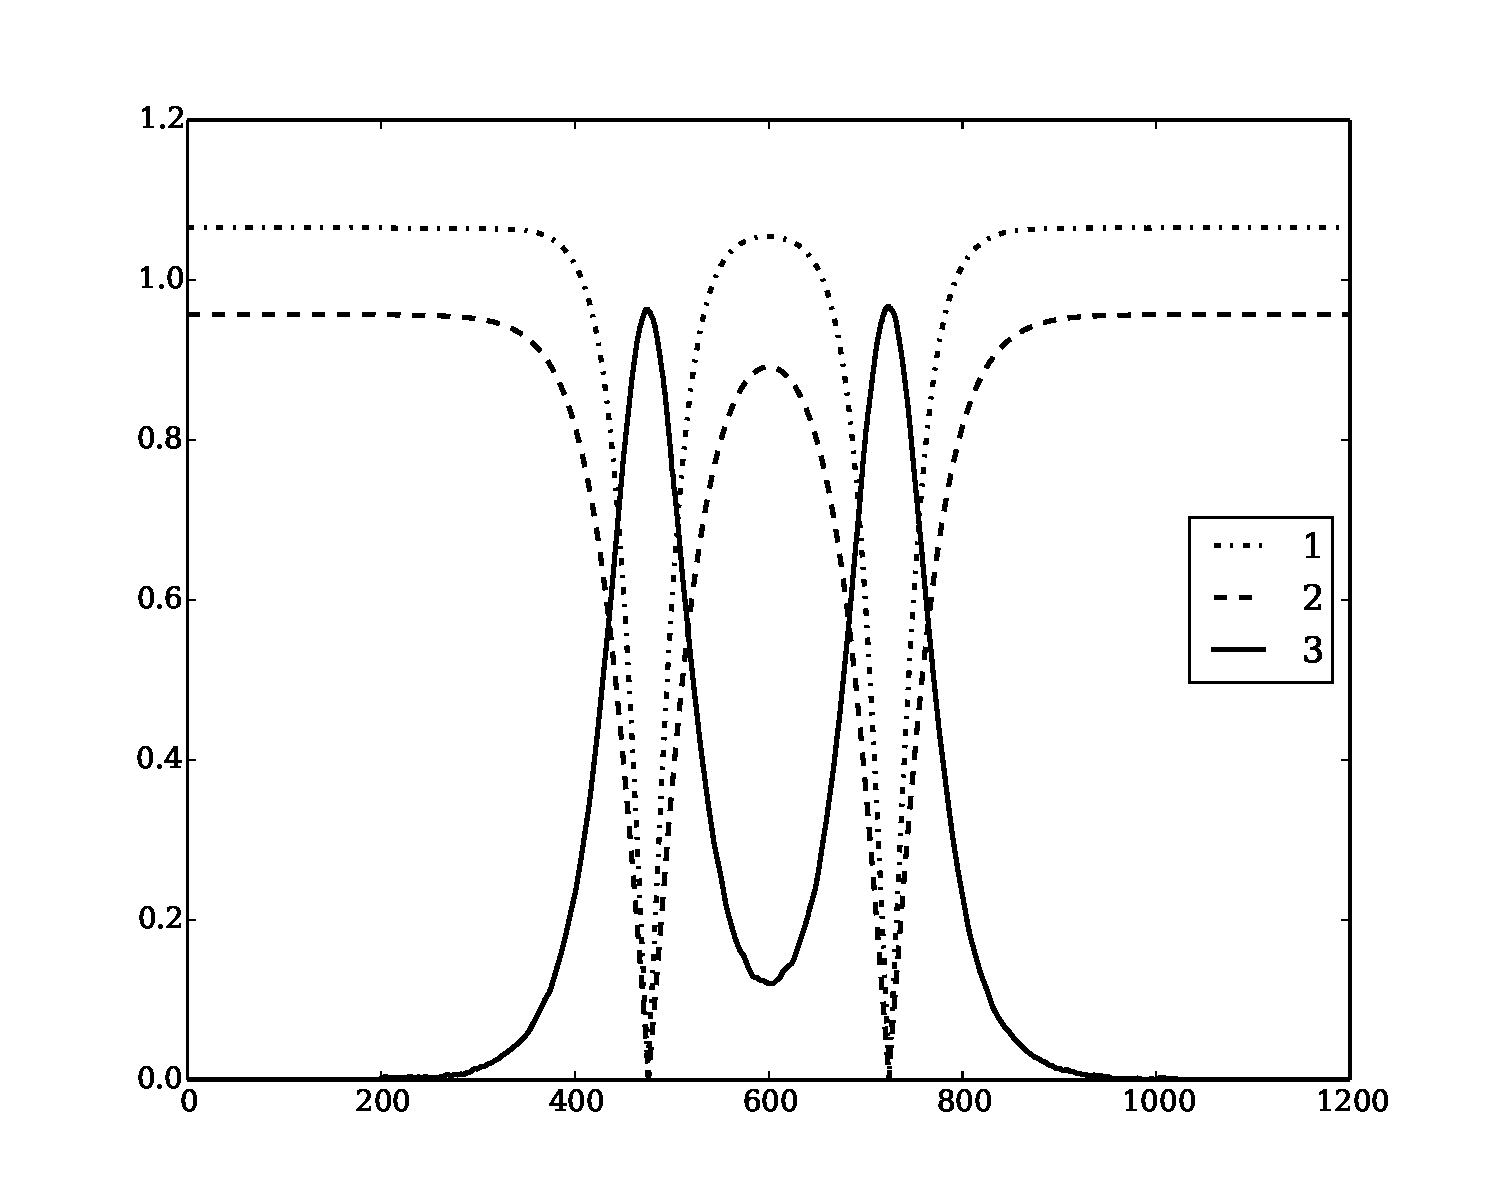
\includegraphics[width=0.5\linewidth]{band_profile}
        % \caption{}
    \end{figure}
\end{frame}